\documentclass[../mcmpaper]{subfiles}
\begin{document}
\section{The Establishment and Solution of the Model of Question 3}
\subsection{Overall Analysis}
By the question, the data of 1/4 bus and subway mobile payment equipment installed after trial operation phase data, because the data can't distinguish between public transit and subway when payment, therefore, this question is no longer consider the specific differences between subway and bus.If it is necessary to estimate all the public transport in the city and realize the profit after payment by the third-party platform of public transport, the following procedures shall be followed:\\
% \begin{figure}[!ht]
% \centering
% 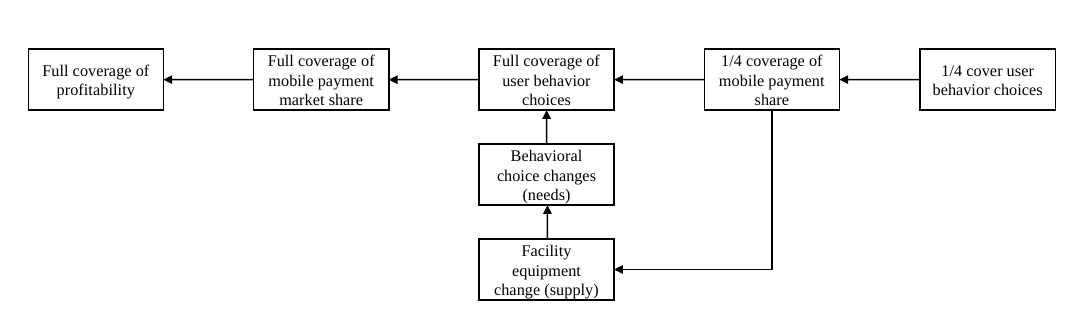
\includegraphics[scale=0.8]{17}
% \caption{Problem three analysis flow chart}
% \end{figure}
\begin{minipage}{1.0\linewidth}
\centering
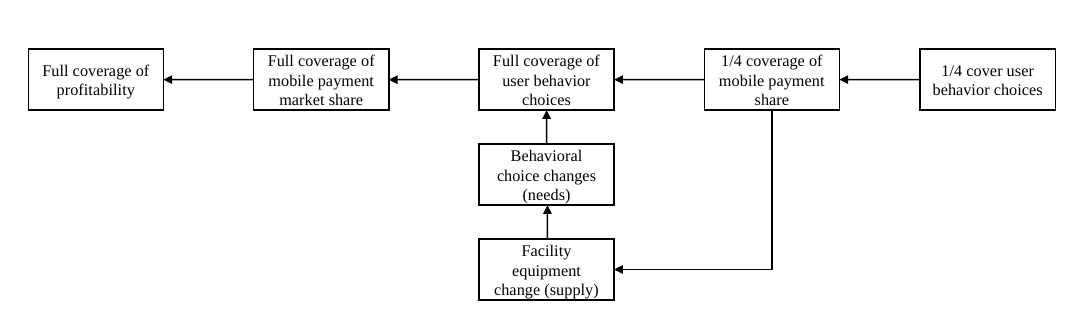
\includegraphics[scale=0.8]{17}
\captionof{figure}{Problem three analysis flow chart}
\end{minipage}\\[1em]
Full coverage Profitability  Full coverage Mobile payment share  Full coverage User behavior choice  1/4 Covered user behavior choice  1/4 covered Mobile payment share Behavior choice Change (demand)  Change of facilities and equipment (supply).
\par
If want to know all the cover under the condition of profit, you need to learn the whole mobile payment under the condition of share.Mobile payment share is closely related to user behavior choice, which is one of the forms of demand.The change of coverage rate is reflected by the change of facilities and equipment, which is the supply part of the system, and the change of supply will affect the demand.Therefore, we need to establish a model to describe the change of behavior choice through the data of mobile payment occupancy and occupancy under the coverage condition of the existing problem no. 14, so as to predict the mobile payment occupancy under the full coverage condition, and then obtain the profitability under the full coverage condition through the model established under the second problem.
\subsection{Analysis of the Current Situation of the Problem-occupancy Rate}
From the data analysis results of question 1, it can be seen that in the case of 1/4 of the mobile payment device, the ratio of the number of mobile payments to the number of bus card payments is about 1, that is, without considering other payment methods, mobile payments account for about 50\%. Therefore, when considering only vehicles with installed equipment, mobile payments must account for more than 50\% of these vehicles. To determine the specific share of mobile payment devices on installed devices, it is necessary to estimate the proportion of passenger traffic of 1/4 covered vehicles to total passenger traffic. By assuming that a quarter of the buses and subways installed with mobile payment devices are the most popular routes in the city, taking Zhengzhou as an example, the passenger flow of the bus lines is sorted from small to large, and the daily passenger flow distribution curve of the line is drawn. After correction, the curve is shown in the Figure~\ref{fig:6.1} and Figure~\ref{fig:6.2}.
\begin{figure}[!ht]
\centering
\begin{minipage}[c]{0.48\linewidth}
    \centering
    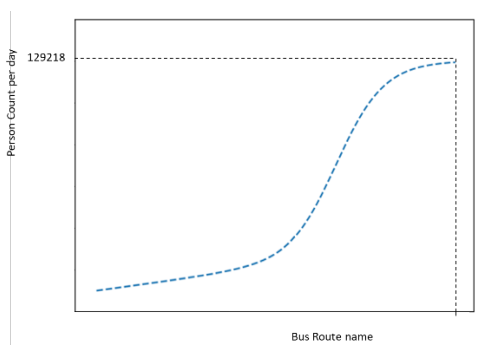
\includegraphics[scale=0.3]{18}
    \caption{Cumulative distribution of bus passenger flow}
    \label{fig:6.1}
\end{minipage}
\quad
\begin{minipage}[c]{0.48\linewidth}
    \centering
    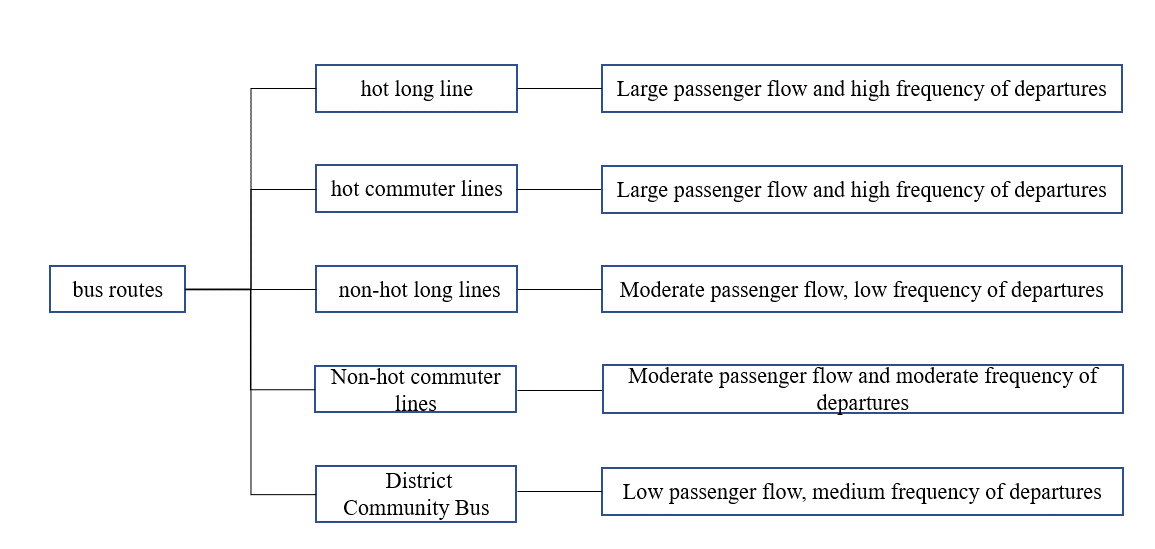
\includegraphics[scale=0.2]{19}
    \caption{Schematic diagram of bus classification}
     \label{fig:6.2}
\end{minipage}
\end{figure}
\par
In the Figure~\ref{fig:6.1}, the horizontal axis represents the bus routes in the city, and the vertical axis is the corresponding daily average passenger flow. After calculation, the bus passenger flow with the top 1/4 passenger flow accounts for about 74.86\% of the total passenger flow. Here it is calculated as 75\%. This is mainly because bus lines can be divided into five types according to coverage and popularity: hot long-distance lines, hot commuter lines, non-hot long-term lines, non-hot commuter lines and community buses in the area. , but the breadth of line distribution is indispensable, resulting in a situation where a small number of lines share a large amount of passenger flow.
\begin{figure}[!ht]
\centering
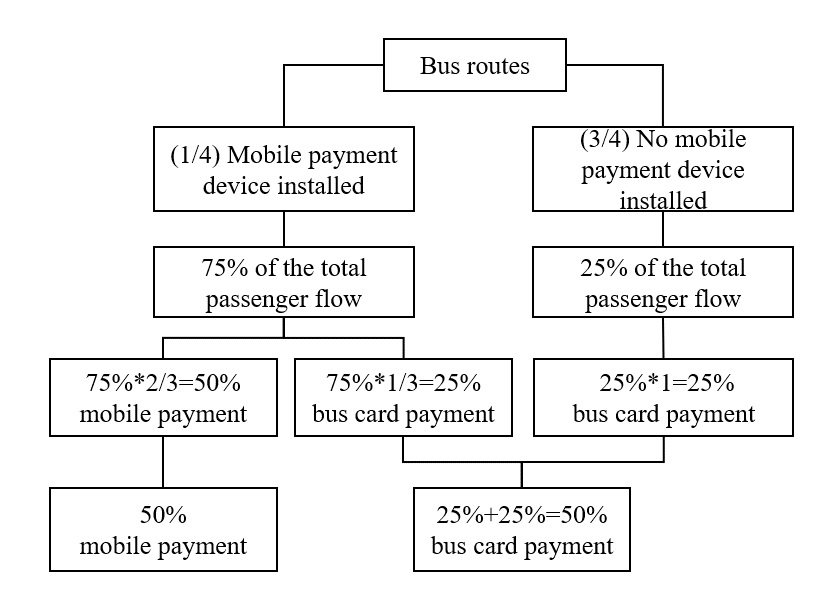
\includegraphics[scale=0.4]{20}
\caption{Mobile payment-bus card payment ratio}
\label{fig:6.3}
\end{figure}
\par
In Figure~\ref{fig:6.3}, it can be seen from the above analysis that in 1/4 of the buses with mobile payment devices installed, mobile payment accounts for 66.6\%, and bus card payment accounts for 33.3\%.
\par
Due to the influence of the supply-demand relationship, the above proportions will change. The supply-demand change relationship is shown in the following Figure~\ref{fig:6.4}:\\
\begin{minipage}{1.0\linewidth}
\centering
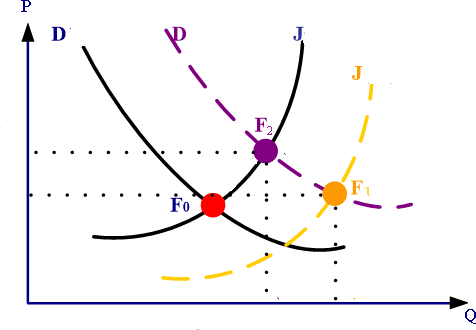
\includegraphics[scale=0.4]{21}
\captionof{figure}{Schematic diagram of changes in supply and demand curves}
\label{fig:6.4}
\end{minipage}
% \begin{figure}[!ht]
% \centering
% 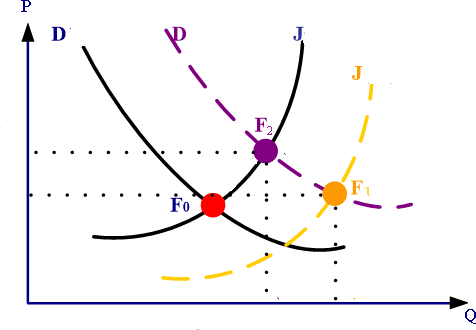
\includegraphics[scale=0.4]{21}
% \caption{Schematic diagram of changes in supply and demand curves}
% \label{fig:6.4}
% \end{figure}
\par
In the initial state, supply and demand are shown by the black curve in the figure, $F_0$ is in equailibium, as the supply increases (the black $J$ curve moves to the right of the yellow dotted line), the demand also changes (the black $D$ curve moves to the right to the purple curve). Therefore, next, the user's choice after full coverage of the device is analyzed from the perspectives of aggregate and non-aggregate.
\subsection{Aggregate Method --- Innovation Diffusion Model}
The innovation diffusion model is based on the innovation diffusion theory, which was proposed by E.M.Roger. Innovation is defined as: an idea, time, or thing considered novel by an individual or other unit of adoption. [1] And innovation has five elements of relative convenience, compatibility, complexity, reliability and perceptibility. The adopters of innovation can be divided into five types: innovators, early adopters, early followers, late followers and laggards. The diffusion pattern of innovation is shown in the following Figure~\ref{fig:6.5} and Figure~\ref{fig:6.6}.\\
\begin{minipage}[c]{\linewidth}
    \centering
    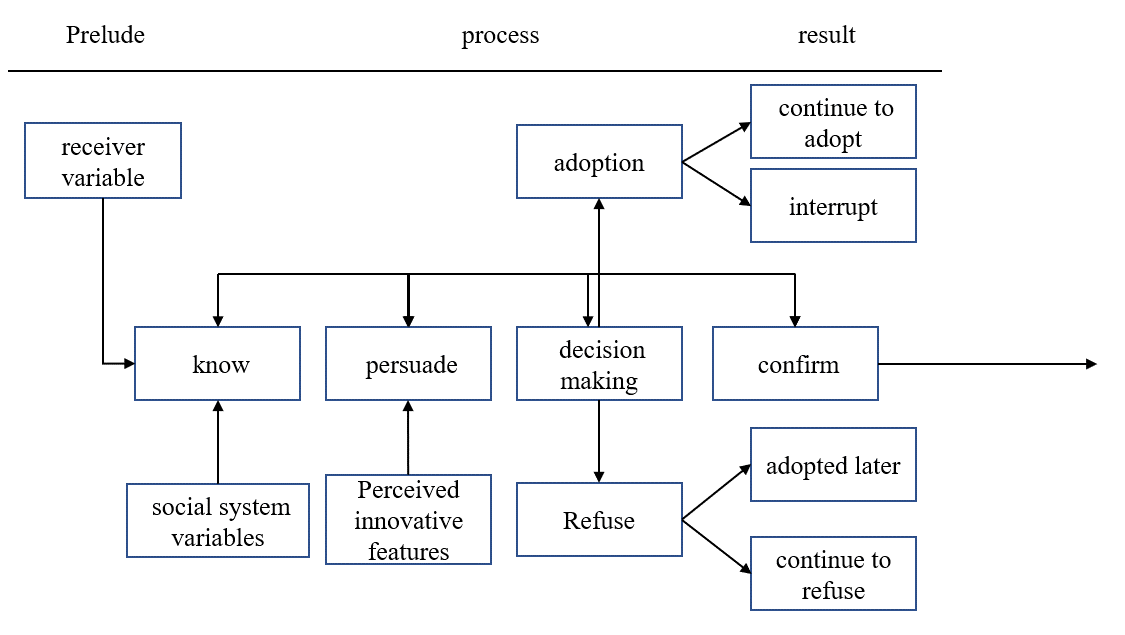
\includegraphics[scale=0.4]{22}
    \captionof{figure}{Roger innovation diffusion model}
    \label{fig:6.5}
\end{minipage}
\par
\begin{figure}[!ht] 
\begin{minipage}[c]{\linewidth}
    \centering
    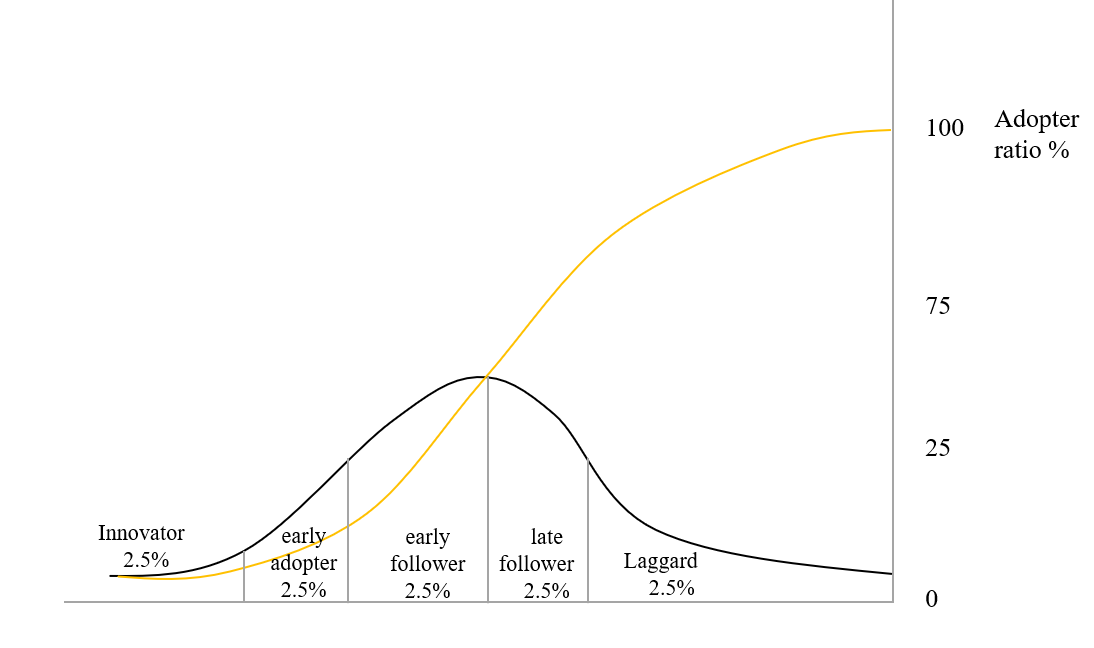
\includegraphics[scale=0.4]{23}
    \caption{Roger innovation diffusion model}
     \label{fig:6.6}
\end{minipage}
\end{figure}
\par
In Figure~\ref{fig:6.6}, the curve shows that in the process of innovation diffusion, about 2.5\% of the people are innovators, 13.5\% are early adopters, 34\% are early followers, 34\% are early followers, and 16\% are early adopters. belong to the laggards.
\par
The process of mobile payment equipment installation and promotion itself is an innovative diffusion process. Using this aggregate model to estimate the full coverage state, the ratio of mobile payers is used. Since the estimation stage is the ratio within a period of time after the equipment is fully covered, so Laggards are not considered here. It is estimated that under the condition of full coverage, 84% of people use mobile payment methods.
\subsection{Disaggregated Methods --- Discrete Choice Models}
Discrete choice model belongs to one of the methods of multivariate analysis, which is a common method of statistical empirical analysis in sociology, biostatistics, quantitative psychology, marketing and so on. This contains: four elements, a decision maker, a finite number of decision options, the attributes of the options, and the preferences of the decision maker. The discrete choice model is based on utility theory, which holds that: \textbf{Model} \ding{173} a decision maker chooses a certain option will get a certain utility \textbf{Model} \ding{173} assuming decision maker rationality and always chooses the option with the greatest utility \textbf{Model} \ding{174} the utility of a certain option is jointly determined by the attributes of that option and the preferences of the decision maker \textbf{Model} \ding{175} the utility has uncertainty, which arises from incomplete knowledge of the decision maker's preferences Incomplete knowledge of the properties of the options.
\par
For this problem, the decision makers, decision options, option properties of this problem are analyzed as follows:
\begin{itemize}[nosep]
    \item Population: young and middle-aged, elderly.
    \item decision options: mobile payment, bus card payment.
    \item Options Properties: actual cost, time of use, equipment coverage, portability, functional breadth, difficulty of use
\end{itemize}
\par
First, analyze the young and middle-aged population, assuming that the utility of each option is a weighted linear combination of attributes, there are:
\begin{equation}
u_{1}=\widehat{u_{1}}+e_{1}=\beta_{6} x_{6}^{1}+\beta_{5} x_{5}^{1}+\beta_{4} x_{4}^{1}+\beta_{3} x_{3}^{1}+\beta_{2} x_{2}^{1}+\beta_{1} x_{1}^{1}+\beta_{0}+e_{1}
\end{equation}
\begin{equation}
u_{2}=\widehat{u_{2}}+e_{2}=\beta_{6} x_{6}^{2}+\beta_{5} x_{5}^{2}+\beta_{4} x_{4}^{2}+\beta_{3} x_{3}^{2}+\beta_{2} x_{2}^{2}+\beta_{1} x_{1}^{2}+\beta_{0}+e_{2}
\end{equation}
Among them, $\mu_{1}$, $\mu_1$ represent the utility of young and middle-aged people to choose mobile payment and bus card payment respectively. $x$ is an attribute, the subscript {1,2,3,4,5,6} corresponds to 6 attributes, and the superscript {1,2} Corresponding to two ways of mobile payment and bus card payment; $\beta$ is a preference parameter, $e$ is a random variable, representing the uncertainty of utility.
\par
According to the theoretical assumptions in the utility theory, the condition for decision makers to choose mobile payment is that the utility of mobile payment is greater than that of bus card payment:
\begin{equation}
\begin{aligned}
u_{1} &>u_{2} \\
\widehat{u_{1}}+e_{1} &>\widehat{u_{2}}+e_{2}
\end{aligned}
\end{equation}
Arranged:
\begin{equation}
\begin{gathered}
e_{1}-e_{2}>\widehat{u_{2}}-\widehat{u_{1}} \\
P_{1}=P\left(u_{1}>u_{2}\right)=P\left(e_{1}-e_{2}>\widehat{u_{2}}-\widehat{u_{1}}\right)
\end{gathered}
\end{equation}
Assuming $e$ is a logistic function, there are:
\begin{equation}
\begin{aligned}
&P_{1}=\frac{e^{\widehat{u_{1}}}}{e^{\widehat{u_{1}}}+e^{\widehat{u_{2}}}} \\
&P_{2}=\frac{e^{\widehat{u_{2}}}}{e^{\widehat{u_{1}}}+e^{\widehat{u_{2}}}}
\end{aligned}
\end{equation}
Under the condition that the equipment coverage is 1/4, it is known from the previous analysis that $P_1=66.6\%, P_2=33.3\%$,quanlity value of $x_1$ to $x_6$ under this condition, and then standardize, the standardization formula is:
\begin{equation}
x^{*}=\frac{x-x_{\min }}{x_{\max }-x_{\min }}
\end{equation}
\par
Using the survey method, preliminarily calculate the preference parameters (ratio between preference parameters) for the young and middle-aged, and bring the calibrated $x$ value, $\beta$ value, and $P$ value into the $P$ value calculation formula, and further adjust the preference parameters to meet the requirements, etc. formula condition.
\par
During the process of expanding the device coverage from 1/4 to 1, the actual cost, access time, portability, functional breadth, and difficulty of use $x_1, x_2, x_3, x_4, x_5, x_6$ attributes do not change, but the device coverage $x_3$ changes. Using the discrete choice model, calculate the probabilities of the young and middle-aged and the elderly choosing two payment methods after expansion, in Table~\ref{tab:7.1}.\\
\begin{minipage}{1.0\linewidth}
\centering
\captionof{table}{Selection probability under full coverage}
\label{tab:7.1}
\begin{tblr}{
      width=\linewidth,
      colspec={X[c]X[c]X[c]},
      hline{1, Z} = {2pt, solid},
      hline{2} = {solid},
      cell{2, 3}{1} = {r=2, b, c}
    }
    decision options & crowd & selection probability \\
    mobile payment & young and middle-aged & 92.17\% \\
    & old age & 25.88\% \\
    bus card payment & young and middle-aged & 7.83\% \\
    & old age & 74.12\% \\
\end{tblr}
\end{minipage}
\par
Using the survey results(Figure~\ref{fig:7.5}) of the characteristics of bus passengers in Zhengzhou City, it can be seen that the elderly (60 years old) account for about 4.1\%, the young and middle-aged (10 years old) account for about 93.3\%, and the rest of the people younger than 10 years old account for less. Here Not be considered. The statistical results are shown in the figure below. After revision, the elderly accounted for 4.2\% and the youth accounted for 95.8\%.
\begin{figure}[htbp]
\centering
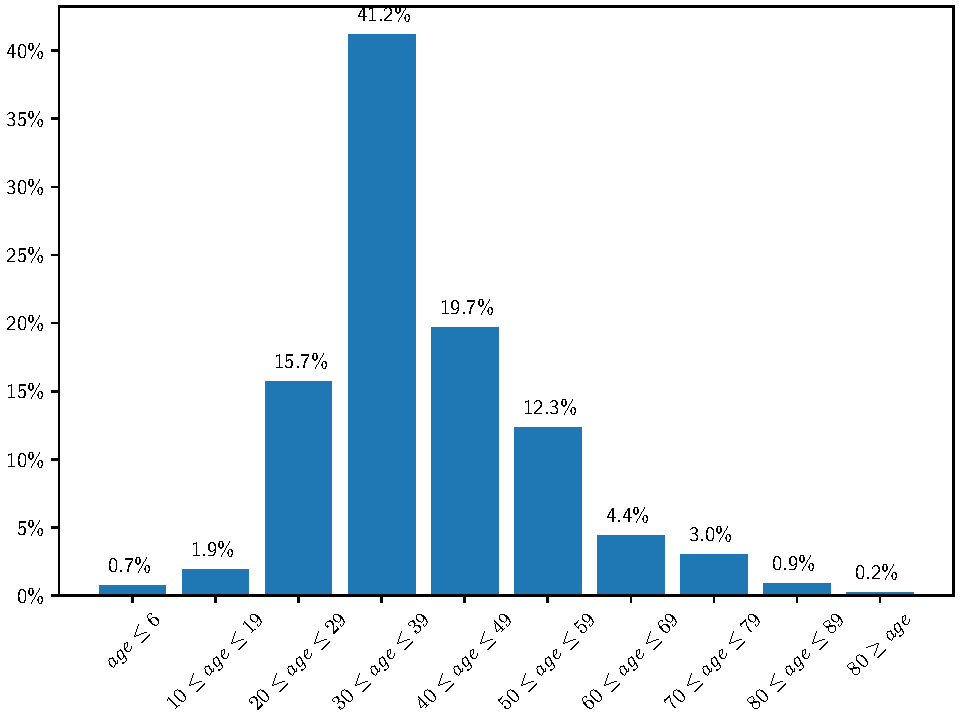
\includegraphics[scale=0.8]{me}
\caption{Age distribution of Zhengzhou bus survey}
\label{fig:7.5}
\end{figure}
\par
Therefore, under the condition of full coverage, the probability of choosing mobile payment is:
\begin{equation}
\begin{aligned}
&P_{1}=\frac{P_{1 y} P_{y}+P_{1 o} P_{o}}{P_{1 y} P_{y}+P_{10} P_{o}+P_{2 y} P_{y}+P_{2 o} P_{o}}=89.50 \% \\
&P_{2}=\frac{P_{2 y} P_{y}+P_{2 o} P_{o}}{P_{1 y} P_{y}+P_{10} P_{o}+P_{2 y} P_{y}+P_{20} P_{o}}=10.50 \%
\end{aligned}
\end{equation}
The subscripts \{1,2\} represent decision-making options (mobile payment, bus card payment), and \{$y, o$\} represent groups (young and middle-aged, elderly).
\subsection{Solving Results}
The aggregate model (innovation diffusion model) and the disaggregated model (discrete choice model) probability results were integrated, and the mean value was calculated. Available: Under the condition of full coverage, the probability of choosing mobile payment is about 86.75\%, and the probability of choosing bus card payment is about 13.25\%.
\par
The selection probability is brought into the second problem model. After calculation, the third-party platform will earn about 7,241,790 yuan per month after full coverage is achieved.
\section{The Solution for the Fourth Question}
\subsection{Business Feasibility Report of Third-party Mobile Payment Platform}
With the continuous progress of industrial level and information technology, smart mobile terminal devices, i.e., smartphones, have entered thousands of households, and third-party mobile payment platforms relying on them have more business opportunities. Combining a third-party mobile payment platform with pre-existing entity magnetic cards, such as: bank cards, car drive cards, membership cards and so on, by partnering with an entity enterprise, and handling fees, service fees, advertising fees as well as precipitation of financial interest are charged for profit during the process of use.
In this question, the third-party payment platform cooperates with the public transportation system to combine the functions of the recharge and use of the ride card with the platform. In the specific business process, the publicity in the early stage, the construction of infrastructure and the labor cost of employees are all increasing with the expansion of the scope of influence. However, the increase in the number of users also expands the profitability of the platform, especially the service fee and precipitation. The growth curve of interest on funds is much higher than the expenditure curve. There are profit models in this article: $W_{0}=I_{0}-O_{0}$, and $f^{\prime}\left(I_{0}\right)>f^{\prime}\left(O_{0}\right) \rightarrow W_{n}-O_{n}>0 \rightarrow W_{n}-O_{n}>W_{n-1}-O_{n-1}$that is, the profit $W$ is growing. In this question, it can be seen that when the platform share increases from 50\% to 86.75\%, the profit increases from 1.9 million to 7.2 million, which is extremely profitable.
\par
Feasibility suggestions for the third-party payment platform:
\begin{itemize}
    \item The third-party payment platform can expand financing and increase the commercial influence and scale of the platform. 
    \item The third-party payment platform can seek multi-faceted cooperation with more entity enterprises.
    \item The third-party payment platform can appropriately reduce the handling fee and attract more customers. 
    \item The third-party payment platform can add a variety of service directions and portable mobile payment channels.
\end{itemize}
\end{document}
%%% Local Variables:
%%% mode: latex
%%% TeX-master: "../mcmpaper"
%%% End:
